\chapter{The Apprehension of Plurality (1987)}

% if we end up needing to add it:
% https://henryflynt.org/studies_sci/reqmath.html

{\centering\itshape
(An instruction manual for 1987 concept art)\par}

\section{Original Stroke-Numerals}

Stroke-numerals were introduced in foundations of mathematics 
by the German mathematician David Hilbert early in the twentieth 
century. Instead of a given Arabic numeral such as `6', for example, one 
has the expression consisting of six concatenated occurrences of the 
stroke, e.g. `$||||||$'. 

To explain the use of stroke-numerals, and to provide a background 
for my innovations, some historical remarks about the philosophy 
of mathematics are necessary. Traditional mathematics had 
treated positive whole-number arithmetic as if the positive whole 
numbers (and geometrical figures also) were objective intangible 
beings. Plato is usually named as the originator of this view. Actually, 
there is a scholarly controversy over the degree to which Plato espoused 
the doctrine of Forms---over whether Aristotle's \booktitle{Metaphysics} put 
words in Plato's mouth---but that is not important for my purposes. 
For an intimation of the objective intangible reality of mathematical 
objects in Plato's own words, see the remarks about "divine" geometric 
figures in Plato's \essaytitle{Philebus.} Aristotle's \booktitle{Metaphysics}, 
1.6, says that mathematical entities 
\begin{quotation}
are intermediate, differing from things perceived in being eternal and 
unchanging, and differing from the Forms in that they exist in copies, 
whereas each Form is unique. 
\end{quotation}

For early modern philosophers such as Hume and Mill, any such 
"Platonic" view was not credible and could not be defended seriously. 
Thus, attempts were made to explain number and arithmetic in ways 
which did not require a realm of objective intangible beings. In fact, 
Hume said that arithmetic consisted of tautologies; Mill that it 
consisted of truths of experience. 

Following upon subsequent developments---the philosophical 
climate at the end of the nineteenth century, and specifically 
mathematical developments such as non-Euclidian geometry---Hilbert proposed 
that mathematics should be understood as a game played with meaningless marks. 
So, for example, arithmetic concerns nothing but formal 
terms---numerals---in a network of rules. Actually, what made arithmetic 
problematic for mathematicians was its infinitary character---as 
expressed, for example, by the principle of complete induction. Thus, 
the principal concern for Hilbert was that this formal game should not, 
as a result of being infinitary, allow the deduction of both a proposition 
and its negation, or of such a proposition as $0=1$. 

But at the same time (without delving into Hilbert's distinction 
between mathematics and metamathematics), the stroke-numerals 
replace the traditional answer to the question of what a number is. The 
stroke-numeral '||||||' is a concrete semantics for the sign `6', and at the 
same time can serve as a sign in place of `6'. The problem of positive 
whole numbers as abstract beings is supposedly avoided by inventing 
e.g. a number-sign, a numeral, for six, which is identically a concrete 
semantics for six. Let me elaborate a little further. A string of six copies 
of a token having no internal structure is used as the numeral `6', the 
sign for six. Thus the numeral is itself a collection which supposedly 
demands a count of six, thereby showing its meaning. Hans Freudenthal 
calls this device an "ostensive numeral." 

So traditionally, there is a question as to what domain of beings 
the propositions of arithmetic refer to, a question as to what the 
referents of number-words are. \emph{Correlative to this, mathematicians' 
intentions require numerous presuppositions about content, and 
require extensive competancies---which the rationalizations for math- 
ematics today are unable to acknowledge, much less to defend.}

For example, if mathematics rests on concrete signs, as Hilbert 
proposed, then, since concrete signs are objects of perception, the 
reliability of mathematics would depend on the reliability of percep- 
tion. Given the script numeral 
{\plainbreak{1}\centering\includegraphics[width=1in]{img/oneortwo}\plainbreak{1}}
which is ambiguous between one and two, conventional mathematics 
would have to guarantee the exclusion of any such ambiguity as this. 
Yet foundations of mathematics excludes perception and the reliability 
of concrete signs as topics---much as Plato divorced mathematics from 
these topics. (Roughly, modern mathematicians would say that reliability 
of concrete signs does not interact with any advanced mathematical 
results. So this precondition can simply be transferred from the requisites 
of cognition in general. But it would not be sincere for Hilbert to 
give this answer. Moreover, my purpose is to investigate the possibility 
of reconstructing our intuitions of quantity beyond the limits of the 
present culture. In this connection, I need to activate the role of 
perception of signs.) 

But the most characteristic repressed presuppositions of mathematics 
run in the opposite, supra-terrestrial direction. Mathematicians' 
intentions require a realm of abstract beings. Again, it is academically 
taboo today to expose such presuppositions.
\footnote{G\"{o}del and Quine admit the need to assume the non-spatial, abstract 
existence of classes. But they cannot elaborate this admission; they cannot 
provide a supporting metaphysics.} But to recur to the 
purpose of this investigation, concept art is about reconstructing our 
intuitions of quantity beyond the limits of the present culture. This 
project demands an account of these repressed presuppositions. To 
compile such an account is a substantial task; I focus on it ina collateral 
manuscript entitled "The Repressed Content-Requirements of Math- 
ematics." To uncover the repressed presuppositions, a combination of 
approaches is required.\footnote{One anthroplogist has written about \enquote{the locus of 
mathematical reality}---but, being an academic, he merely reproduces a stock answer outside 
his field (namely that the shape of mathematics is dictated by the physiology of 
the brain).} I will not dwell further on the matter here---
but a suitable sample of my results is the section "The Reality-Character 
of Pure Whole Numbers and Euclidian Figures" in \emph{The Repressed Content-Requirements.}

Returning to the original stroke-numerals, they were meant 
(among other things) to be part of an attempt to explain arithmetic 
without requiring numbers as abstract beings. They were meant as 
signs, for numbers, which are identically their own concrete semantics. 
Whether I think Hilbert succeeded in dispensing with abstract entities is 
not the point here. I am interested in how far the exercise of positing 
stroke-numerals as primitives can be elaborated. My notions of the 
original stroke-numerals are adapted from Hilbert, Weyl, Markov, 
Kneebone, and Freudenthal. For example, how does one test two 
stroke-numerals for equality? To give the answer that "you count the 
strokes, first in one numeral and then in the other," is not in the spirit of 
the exercise. For if that is the answer, then that means that you have a 
competency, "counting," which must remain a complete mystery to 
foundations of mathematics. What one wants to say, rather, is that you 
test equality of stroke-numerals by "cross-tallying": by e.g. deleting 
strokes alternately from the two numerals and finding if there is a 
remainder from one of the numerals. This is also the test of whether one 
numeral precedes the other. So, now, given an adult mastery of quality 
and abstraction, you can identify stroke-numerals without being able 
to "count." 

In the same vein, you add two stroke-numerals by copying the 
second to the right of the first. You subtract a shorter numeral from a 
longer numeral by using the shorter numeral to tally deletion of strokes 
from the longer numeral. You multiply two stroke-numerals by copying the second as many times as there are strokes in the first: that is, by 
using the strokes of the first to tally the copying of the second numeral. 

To say that all this is superfluous, because we already acquired 
these "skills" as a child, misses the point. The child does not face the 
question, posed in the Western tradition, of whether we can avoid 
positing whole numbers as abstract beings. To weaken the requirements 
of arithmetic to the point that somebody with an adult mastery 
of quality and abstraction can do feasible arithmetic "blindly"---i.e. 
without being able to "count," and without being able to see number-names 
('five', 'seven', etc.) in concrete pluralities---is a notable exercise, 
one that correlates culturally with positivism and with the machine age. 

To reiterate, the stroke-numeral is meant to replace numbers as 
abstract beings by providing number-signs which are their own concrete 
semantics. Freudenthal said that we should communicate positive 
whole numbers to alien species by broadcasting stroke-numerals to 
them (in the form of time-series of beeps). Still, Freudenthal said that 
the aliens would have to resemble us psychologically to get the point.\footnote{\booktitle{Lincos}, pp. 14--15.} 

When Hilbert first announced stroke-numerals, certain difficulties 
were pointed out immediately. It is not feasible to write the 
stroke-numerals for very large integers. (And yet, if it is feasible to write the 
stroke-numeral for the integer n, then there is no apparent reason why 
it would not also be feasible to write the stroke-numeral for n+1. So 
stroke-numerals are closed under succession, and yet are contained in a
finite segment of the classical natural number series.) Moreover, large 
feasible stroke-numerals, such as that for 10,001, are not surveyable. 

But this is not a study of metamathematical stroke-numerals. And 
I do not wish to go into Hilbert's question of the consistency of 
arithmetic as an infinitary game here; "The Repressed Content-Requirements" 
will have more to say on the consistency question. The 
purpose of this manual, and of the artworks which it accompanies, is to 
establish apprehensions of plurality beyond the limits of traditional 
civilizations (beyond the limits of Freudenthal's "us"). Moreover, these 
apprehensions of plurality are meant to violate the repressed presuppo- 
sitions of mathematics. I refer back to original stroke-numerals because 
certain devices which I will use in assembling my novelties cannot be 
supposed to be intuitively comprehensible---certainly not to the 
traditionally-indoctrinated reader---and will more likely be understood 
if I mention that they are adaptations of features of original stroke- 
numerals. Let me mention one point right away. In our culture, we 
usually see numerals as positional notations---e.g. 111 is decimal 
$1\times 10^2+1\times 10^1+1$ or binary $1\times 2^2+1\times 2^1+1$. But stroke-numerals 
are not a positional notation (except trivially for base 1). Likewise, my 
novelties will not be positional notations; I will even nullify the 
reference to base 1. (Only much later in my investigations, when broad 
scope becomes important, will I use positional notation.) So the 
foregoing introduction to stroke-numerals has only the purpose of 
motivating my novelties. And references to the academic canon are given 
only for completeness. They cannot be norms for what I am "permitted" to posit. 

\section{Simple Necker-Cube Numerals}

In my stroke-numerals, the printed figure, instead of being a 
stroke, is a Necker cube. (Refer to the attached reproduction, "Stroke- 
Numeral.") A Necker cube is a two-dimensional representation of a 
cubical frame, formed without foreshortening so that its perspective is 
perceptually equivocal or multistable. The Necker cube can be seen as 
flat, as slanting down from a central facet like a gem, etc.; but for the 
moment I am exclusively concerned with the two easiest variants in 
which it is seen as an ordinary cube, either projecting up toward the 
front or down toward the front. 

{\center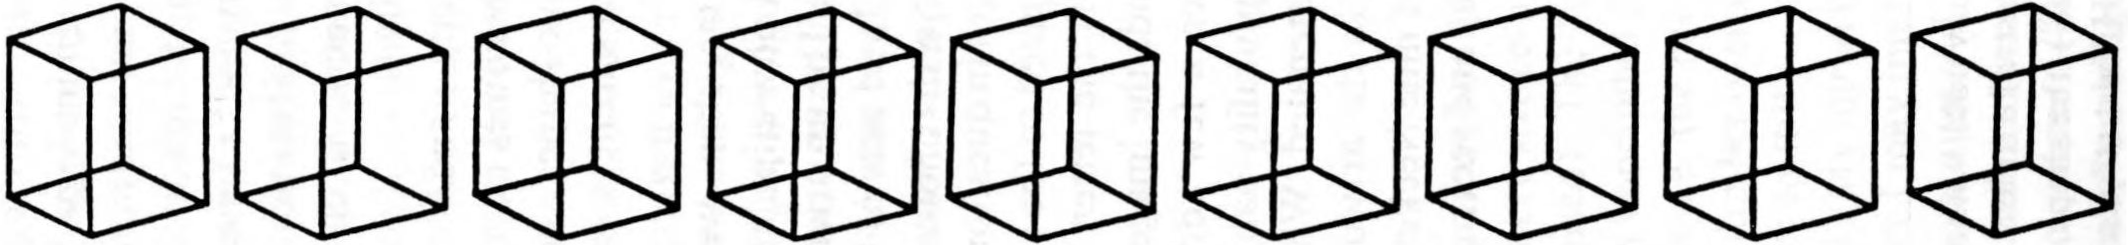
\includegraphics[width=4in]{img/neckercube}\plainbreak{2}
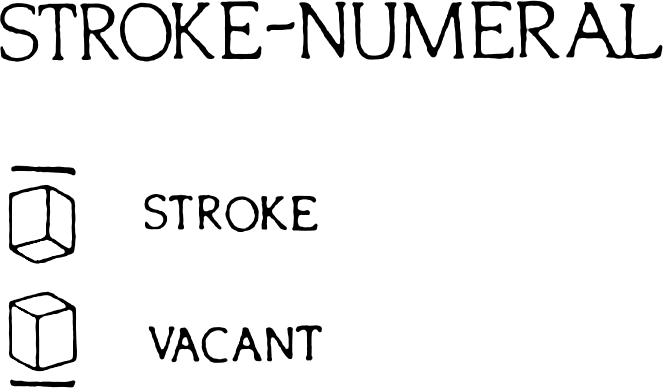
\includegraphics[width=2in]{img/neckerkey}\par}

Since I will use perceptually multistable figures as notations, I 
need a terminology for distinctions which do not arise relative to 
conventional notation. I call the ink-shape on paper a \term{figure}. I call the 
stable apparition which one sees in a moment---which has imputed 
perspective---the \term{image}.\footnote{I may note, without wanting to be precious, that a bar does not count as a Hilbert stroke unless it is vertical relative to its reader.}
As you gaze at the figure, the image changes 
from one orientation to the other, according to intricate subjective 
circumstances. It changes spontaneously; also, you can change it 
voluntarily. 

Strictly---and very importantly---it is the image which in this 
context becomes the notation. Thus, I will work with notations which 
are not ink-shapes and are not on a page. They arise as active interactions 
of awareness with an "external" or "material" print-shape or 
object. 

So far, then, we have images---partly subjective, pseudo-solid 
shapes. I now stipulate an alphabetic role for the two orientations in 
question. The up orientation is a \term{stroke}; the down orientation is called 
"\term{vacant}," and acts as the proofreaders' symbol $\closure$, meaning "close up space." 
(So that "vacant" is not "even" an alphabetic space.) Now the 
two images in question are \term{signs}. The transition from image to sign can 
be analogized to the stipulation that circles of a certain size are (occurances 
of) the letter "o."\footnote{And---the shape, bar, positioned vertically relative to its reader, is the symbol, Hilbert stroke.} I may say that one sees the image; one 
apprehends the image as sign. 

When a few additional explanations are made, then the signs 
become plurality-names or "numerals." First, figures, Necker cubes, 
are concatenated. When this is done, a display results. So the 
stroke-numeral in the artwork, as an assembly of marks on a surface, is a 
display of nine Necker cubes. An image-row occurs when one looks at 
the display and sees nine subjectively oriented cubes, for just so long as 
the apparition is stable (no cube reverses orientation). I chose nine 
Necker cubes as an extreme limit of what one can apprehend in a fixed 
field of vision. (So one must view the painting from several meters 
away, at least.) The reader is encouraged to make shorter displays for 
practice. Incidentally, if one printed a stroke-numeral so long that one 
could only apprehend it serially, by shifting one's visual field, it would 
be doubtful that it was well-defined. (Or it would incorporate a feature 
which I do not provide for.) The universe of pluralities which can be 
represented by these stroke-numerals is "small." My first goal is to 
establish "subjectified" stroke-numerals at all. They don't need to be 
large. 

The concatenated signs which you apprehend in a moment of 
looking at the display are now apprehended or judged as a 
plurality-name, a numeral. At the level where you apprehend signs (which, 
remember, are alphabetized, partly subjective images, not figures), the 
apparition is disambiguated. Thus I can explain this step of judging the 
signs as plurality-names by using fixed notation. For nine Necker cubes 
with the assigned syntactical role, you might apprehend such 
permutations of signs as 
\begin{enumerate}[label=\alpha*.]
	\item $|\closure\closure||\closure\closure\closure|$
	\item $|\closure\closure\closure\closure\closure|||$
	\item $||||\closure\closure\closure\closure\closure$
	\item $||||\closure\closure\closure\closure|$
	\item $\closure\closure\closure\closure\closure\closure\closure\closure\closure$
\end{enumerate}

My Necker-cube stroke-numerals are something new; but (a)--(e) are 
not---they are just a redundant version of Hilbert stroke-numerals 
(which nullifies the base 1 reference as I promised). The "close up 
space" signs function as stated; and the numeral concluded from the 
expression corresponds to the number of strokes; i.e. the net result is 
the Hilbert stroke-numeral having the presented number of strokes. So 
(a) and (b) and (c) all amount to $|||$. (d) amounts to $|||||$.

As for (e), it has the alphabetic role of a blank. My initial interpretation 
of this blank is "no numeral present." Later I may interpret the 
blank as "zero," so that every possibility will be a numeral. Let me 
explain further. Even when I will interpret the blank as "zero." it will 
not come about from having nine zeros mapped to one zero (like a sum 
of zeros). (e) has nine occurrences of "close up space," making a blank. 
There is always only one way of getting "blank." (A two-place display 
allows two ways of getting "one" and one way of getting "two"; etc.) 
The notation is not positional. It is immaterial whether one "focuses" 
starting at the left or at the right. 

Relative to the heuristic numerals (a)--(e), you may judge the 
intended numerals by counting strokes, using your naive competency 
in counting. (It is also possible to use such numerals as (a)--(e) "blindly" 
as explained earlier. This might mean that there would be no recognition 
of particular numbers as gestalts; identity of numbers would be
handled entirely by cross-tallying.) The Necker-cube numerals, however, 
pertain to a realm which is in flux because it is coupled to 
subjectivity. My numerals provide plurality-names and models of that 
realm. Thus, the issue of what you do when you conclude a numeral 
from a sign in perception is not simple. \emph{We have to consider different 
hermeneutics for the numerals---and the ramifications of those hermeneutics.}
Here we begin to get a perspective of the mutability which my 
devices render manageable. 

For one thing, given a (stable) image-row, and thus a sign-row, you 
can indeed use your naive arithmetical competency to count strokes, 
and so conclude the appropriate numeral. This is \term{bicultural hermeneutic}, 
because you are using the old numbers to read a new notation for 
which they were not intended. We use the same traditional counting, of 
course, to speak of the number of figures in a display. 

(This prescription of a hermeneutic is not entirely straightforward. 
The competency called counting is required in traditional mathematics. 
But such counting is already paradoxical "phenomenologically." I 
explain this in the section called "Phenomenology of Counting" in \essaytitle{The 
Repressed Content-Requirements}. As for the Necker-cube numerals, 
the elements counted are not intended in a way which supports the 
being of numbers as eternally self-identical. So the Necker-cube 
numerals might resonate with the phenomenological paradoxes of 
ordinary counting. The meaning of ordinary numbering, invoked in 
this context, might begin to dissolve. But I mention this only to hint at 
later elaborations. At this stage, it is proper to recall one's inculcated 
school-counting; and to suppose that e.g. the number of figures in a 
display is fixed in the ordinary way.) 

Then, there is the \term{ostensive hermeneutic}. Recall that I explained 
Hilbert stroke-numerals as signs which identically provide a concrete 
semantics for themselves; and as an attempt to do arithmetic without 
assuming that one already possesses arithmetic in the form of competency 
in counting, or of seeing number-names in pluralities. My 
intention was to prepare the reader for features to be explained now. 
On the other hand, at present we drop the notion of handling identity of 
numerals by cross-tallying.\footnote{Because this notion corresponds to a situation in which we are unable to appraise image-rows as numerals, as gestalts.}
For the ostensive hermeneutic, it is crucial 
that the display is short enough to be apprehended in a fixed field of 
vision. 

With respect to short Hilbert numerals, I ask that when you see 
e.g. 

$$||$$

marked ona wall, you grasp it asa sign for a definite plurality, without 
mediation---without translating to the word "two." A similar intention 
is involved in recognizing 
$$\sout{||||}$$
as a definite plurality, as a gestalt, without translating to "five." 

Now I ask you to apply this sort of hermeneutic to Necker-cube 
stroke-numerals. I ask you to grasp the sign-row as a numeral, as a 
gestalt. (Without using ordinary counting to call off the strokes.) Fora 
two-place display, you are to take such images as 

\newcommand{\neckup}{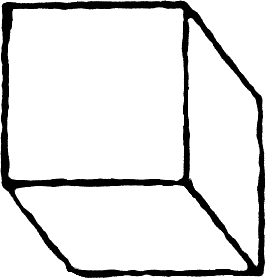
\includegraphics[width=1in]{img/neckerup}}
\newcommand{\neckdown}{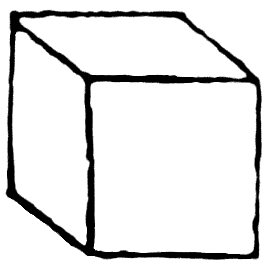
\includegraphics[width=1in]{img/neckerdown}}

{\centering\neckup\neckdown\par}
and
{\centering\neckup\neckup\par}
as plurality-names without translating into English words. (Similarly 

{\centering\neckdown\neckdown\par}

in the case where I choose to read "blank" as "zero.") Perhaps it is 
necessary to spend considerable time with this new symbolism before 
recognition is achieved. Again, I encourage the reader to make short 
displays for practice. I have set a display of nine figures as the upper 
limit for which it might be possible to learn to grasp every sign-row as a 
numeral, as a gestalt. 

The circumstance that the apprehended numeral may be different 
the next moment is not a mistake; the apprehended numeral is supposed 
to be in flux. So when you see image-rows, you take them as 
identical signs/semantics for the appearing pluralities. 

But who wants such numerals---where are there any phenomena 
for them to count? For one thing, they count the very image-rows which 
constitute them. The realm of these image-rows is a realm of subjective 
flux: its plurality is authentically represented by my numerals, and 
cannot be authentically represented by traditional arithmetic. 

A further remark which may be helpful is that here numerals arise 
only visually. So far, my numerals have no phonic or audio equivalent. 
(Whereas Freudenthal in effect posited an audio version of Hilbert 
numerals, using beeps.) 

To repeat, by the "ostensive hermeneutic" I mean grasping the 
sign-row, without mediation, as a numeral. But there is, as well, the 
point that the Necker-cube numerals are \term{ostensive numerals}. That is, 
the (momentary) numeral for six would in fact be an image-row with 
just six occurrences of the image "upward cube." (Compare e.g. 
$|||\closure\closure||\closure|$) The numeral is a collection in which only the "copies" of 
"upward cube" contribute positively, so to speak; and these copies 
demand a count of six (bicuturally). This feature needs to be clear, 
because later I will introduce numerals for which it does not hold. 

Let me add another proviso concerning the ostensive hermeneutic 
which will be important later. I will illustrate the feature in question 
with an example which, however, is only an analogy. Referring to 
Arabic decimal-positional numerals, you can appraise the number-name of 
$$1001$$
(comma omitted) immediately. But consider 
$$786493015201483492147$$
Here you cannot appraise the number-name without mediation. That 
is, if you are asked to read the number aloud, you don't know whether 
to begin with "seven" or "seventy-eight" or "seven hundred eighty-six." 
Lacking commas, you have to group this expression from the right, in 
triples, to find what to call it. An act of analysis is required. 

In the case of Necker-cube numerals and the ostensive hermeneutic, 
I don't want you to see traditional number-names in the pluralities. 
However, I ask you to grasp a sign-row as a numeral, as a gestalt. I now 
add that the gestalt appraisal is definitive. I rule out appraising image-rows 
analytically (by procedures analogous to mentally grouping an 
Arabic number in triples). (I established a display of nine figures as the 
upper limit to support this.) 

The need for this proviso will be obscure now. It prepares for a 
later device in which, even for short displays, gestalt appraisal and 
appraisal by analysis give different answers, either of which could be 
made binding. 

\breatk

The bicultural hermeneutic is applied, in effect, in my uninterpreted 
calculus \textsc{"Derivation,"} which serves as a simplified analogue of 
my early concept art piece \textsc{"Illusions."} (Refer to the reproductions on 
the next four pages.) Strictly, though, "Derivation" does not concern a 
Necker-cube stroke-numeral. The individual figures are not Necker 
cubes, but "Wedberg cubes," formed with some foreshortening to make 
one of the two orientations more likely to be seen than the other. What 
is of interest is not apprehension of image-rows as numerals, but rather 
appraisal of lengths of the image-rows via ordinary counting. As for the 
lessons of this piece, a few simple observations are made in the piece's 
instructions. But to pursue the topic of concept art as uninterpreted 
calculi, and derive substantial lessons from it, will require an entire 
further study---taking off from earlier writings on post-formalism and 
uncanny calculi, and from my current writings collateral to this essay. 


1987 Concept Art --- Henry Flynt 
"DERIVATION" (August 1987 corrected version) 


Purpose: To provide a simplified analogue of my 1961 concept art piece "'IIlusions'' which is 
discrete and non-''warping.''* Thereby certain features of "'Illusions'' become more 
clearly discernible. 


Given a perceptually multistable figure, the ""Wedberg cube," which can be seen in two 
orientations: as a cube; as a prism (trapezohedron.) 

Call what is seen at an instant an /mage. 

Nine figures are concatenated to form the display. 


An element is an image of the display for as long as that image remains constant (Thus, 
elements include: the image from the first instant of a viewing until the image first 
changes; an image for the duration between two changes; the image from the last 
change you see in a viewing until the end of the viewing.) 


The /ength of an element equals the number of prisms seen. Lengths from O through nine 
are possible. Two different elements can have the same length. Length of element X 
is written /(X). 


Elements are seen in temporal order in the lived time of the spectator. | refer to this order by 
words with prefix 'T'. T-first; T-next; etc. 


Element Y succeeds element X if and only if 
i) (X) = KY), and Y is T-next after X of all elements with this length; or 
ii) ¥ is the T-earliest element you ever see with length /(X) + 1. 
Note that (ii) permits Y to be T-earlier than X: the relationship is rather artificial. 


The initial element A is the T-first element. (/(A) may be greater than O; but it is likely to be O 
because the figure is biased.) 


The conclusion C is the T-earliest element of length 9 (exclusive of Ain the unlikely case in 
which /(A) = 9). 


A derivation is a series of elements in lived time which contains A and C and in which every 
element but A succeeds some other element. 


Discussion 

To believe that you have seen a derivation, you need to keep track that you see each 
possible length, and to force yourself to see lengths which do not occur spontane- 
ously. 


You may know that you have seen a derivation, without being able to identify in memory the 
particular successions. 


"Derivation" is not isomorphic to "Illusions" for a number of reasons. ''Illusions" doesn't 
require you to see individually every possible ratio between the T-first ratio and unity. 
"Illusions" allows an element to succeed itself. The version of 'Derivation' pres- 
ented here is a compromise between mimicking "'Illusions"' and avoiding a trivial or 
cluttered structure. Any change such as allowing elements to succeed themselves 
would require several definitions to be modified accordingly. 


*In "Illusions," psychic coercion, which may be called "false seeing" or "warping," is 
recommended to make yourself see the ration as unity. In ''Derivation," this warping is not 
necessary; all that may be needed is that you see certain lengths willfully. 


ABABA AAS 


Concept Art Version of Mathematics System 3/26/6l(6/19/61) 

An "element"is the facing page (with the figure on it) so long 
as the apparent, perceived, ratio of the length of the vertical 
line to that of the horizontal line (the element's "associated 
ratio") does not change. 

A "selection sequence" is asequence of elements of which the 
first is the one having the greatest associated ratio, and 
each of the others has the associated ratio next smallerthan 
that of the preceding one. (To decrease the ratio, come to 
see the vertical line as shorter, relative to the horizontal 
line, one might try measuring the lines with a ruler to con- 
vince oneself that the vertical one is not longer than the 
other, and then trying to see the lines as equal in length; 
constructing similar figures with a variety of real (measured) 
ratios and practicing judging these ratios; and so forth.) 
(Observe that the order of elements in a selection sequence 
may not be the order in which one sees them.] 


An elaboration of "Stroke-Numeral" should be mentioned here, 
the piece called "an Impossible Constancy." (Refer to the facing page.) 
As written, this piece presupposes the bicultural hermeneutic, and that 
is probably the way it should be formulated. The point of this piece, 
paradoxically, is that one seeks to annul the flux designed into the 
apprehended numeral. Viewing of the Necker-cube numeral is placed 
in the context of a lived experience which is interconfirmationally 
weak: namely, memory of past moments within a dream (a single 
dream). Presumably, appraisals of the numeral at different times could 
come out the same because evidence to the contrary does not survive. 
So inconstancy passes as constancy. Either hermeneutic can be 
employed; but when I explained the hermetic hermeneutic, I encour- 
aged you to follow the flux. Here you wouldn't do that---you wouldn't 
stare at the display over a retentional interval. 


As for the concept of equality with regard to Necker-cube numerals, 
what can be said about it at this point? We have equality of numbers of 
figures in displays, by ordinary counting. We have two hermeneutics 
for identifying an apprehended numeral. In the course of expounding 
them, I expounded equivalence of different permutations of "stroke" 
and "vacant." Nevertheless, given that, for example, a display of two 
figures can momentarily count the numeral apprehended from a dis- 
play of three figures,* we are in unexplored territory. Cross-tallying, 
suitable for judging equality of Hilbert numerals, seems maladapted to 
Necker-cube numerals; in fact, I dismissed it when introducing the 
ostensive hermeneutic. 

If the "impossible constancy" from the paragraph before last were 
manageable, then one might consider restricting the ultimate definition 
of equality to impossible constancies. That is, with respect to a single 
display, if one wanted to investigate the intention of constancy (self- 
equivalence of the apprehended numeral), one might start with the 
impossible constancy. Appraisals of a given display become constant 
(the numeral becomes self-equivalent) in the dream. Then two displays 
which are copies might become constantly equivalent to each other, in 
the dream. 

Such is a possibility. To elaborate the basics and give an incisive 
notion of equality is really an open problem, though. Other avenues 
might require additional devices such as the use of figures with distinc- 
tions of appearance. 


*that it is not assured that copies of a numeral will be apprehended or 
appraised correlatively 


1987 Concept Art --- Henry Flynt 
Necker-Cube Stroke-Numeral: AN IMPOSSIBLE CONSTANCY 


The purpose of this treatment is to say how a Necker-cube stroke numeral may be 
judged (from the standpoint of private subjectivity) to have the same value at different 
times; even though the conventional belief-system says that the value is likely to change 
frequently. 


This is accomplished by selecting a juncture in an available mode of illusion, namely 
dreaming, which annuls any distinction between an objective circumstance, and the 
circumstance which exists according to your subjective judgment. In the first instance, | 
don't ask you to change your epistemology. Instead, to repeat, | select an available juncture 
in lived experience at which the conventional epistomology gets collapsed. 


You have to occupy yourself with the stroke-numeral to the point that you induce 
yourself to dream about it. 

When, in apprehending a stroke-numeral, you "judge" the value of the numeral, the 
number, this refers to the image you see and to the number-word which you may conclude 
from the image. 

Suppose that in a single dreamed episode, you judge the value of the numeral at two 
different moments. Suppose that at the second moment, you do not register any discre- 
pancy between the value at the second moment and what the value was at the first 
moment. Then you are permitted to disregard fallibility of memory, and to conclude that the 
values were the same at both moments: because if your memory has changed the past, it 
has done so tracelessly. A tracelessly-altered past may be accepted as the genuine past. 


Refinements. The foregoing dream-construct may be "'lifted" to waking experience, as 
per the lengthy explanations in ""An Epistemic Calculus."' Now you are asked to alter your 
epistemology, selectively to suspend a norm of realism. 

Now that we are concerned with waking experience, a supporting refinement is 
possible. Suppose | make an expectation (which may be unverbalized) that the value of the 
numeral at a future moment will be the same that it is now. This expectation cannot be 
proved false, if: the undetermined time-reference 'future moment" is applied only at those 
later moments when the value is the same as at the moment the expectation was made. 
(Any later moment when the value is not the same is set aside as not pertinent, or forgotten 
at still later moments when the value is the same.) 


As a postscript, there is another respect in which testing a fact requires trust in a 
comparable fact. Suppose | make a verbalized expectation that the value of the numeral in 
the future will be the same as at present. Then to test this expectation in the future depends 
on my memory of my verbalization. My expectation cannot be belied unless | have a sound 

"memory that the number | verbalized in my expectation is different from the number | 
conclude from the image now. 


HT. Inconsistently-Valued Numerals 


As the "Wedberg cube" illustrates, a cubical frame can be formed 
in different ways, altering the likelihood that one or another image is 
seen. With respect to the initial uses of the Necker-cube stroke-numeral 
a figure is wanted which lends itself to the image of a cube projecting 
up, or of a cube projecting down, with an approximately equal likeli- 
hood for the two images---and which makes other images unlikely. 
Now let a Necker cube be drawn large, with heavy line-segments, with 
all segments equally long, with rhomboid front and back faces; and 
display it below eye level. 


As you look for the up and down orientations, there should be 
moments when paradoxically you see the figure taking on both of these 
mutually-exclusive orientations at once---yielding an apparition which 
is a logical/ geometric impossibility. The sense-content in this case is 
dizzying. 

That we have perceptions of the logically impossible when we 
suffer illusions has been mentioned by academic authors. (Negative 
afterimages of motion---the waterfall illusion.) Evidently, though, these 
phenomenaare so distasteful to sciences which are still firmly Aristote- 
lian that the relations of perception, habituation, language, and logic 
manifested in these phenomena have never been assessed academically. 
For me to treat the paradoxical image thoroughly here would be too 
much of a digression from our subject, the apprehension of plurality. 
However, a sketchy treatment of the features of the impossible image is 
necessary here. 

To begin with, the paradoxical image of the Necker cube is not the 
same phenomenon as the "impossible figures" shown in visual percep- 
tion textbooks. The latter figures employ "puns" in perspective coding 
such that parts of a figure are unambiguous, but the entire figure 


cannot be grasped as a gestalt coherently. Then, the paradoxical Necker- 
cube image is not an inconsistently oriented object (as the reader may 
have noted). It is an apparitional depiction of an inconsistently oriented 
object. But this is itself remarkable. For since a dually-oriented cube (in 
Euclidean 3-space) is self-contradictory by geometric standards, a 
picture of it amounts to a non-vacuous semantics for an inconsistency. 
Another way of saying the same thing is that the paradoxically- 
oriented image is real as an apparition. 

If one is serious about wanting a "logic of contradictions"---a logic 
which admits inconsistencies, without a void semantics and without 
entailing everything---then one will not attempt to get it by a contorted 
weakening of received academic logic. One will start from a concrete 
phenomenon which demands a logic of contradictions for its authentic 
representation---and will let the contours of the phenomenon shape the 
logic. 

In this connection, the paradoxically-oriented Necker-cube image 
provides a lesson which I must explain here. Consider states or proper- 
ties which are mutually exclusive, such as "married" and "bachelor." 
Their conjunction---in English, the compound noun "married 
bachelor"---is inconsistent.* On the other hand, the joint denial 
"unmarried nonbachelor" is perfectly consistent and is satisfied by 
nonpersons: a table is an unmarried nonbachelor. "Married" and 
"bachelor" are mutually exclusive, but not exhaustive, properties. Only 
when the domain of possibility, or intensional domain, is restricted to 
persons, so "married" and "bachelor" become exhaustive properties. ** 
Then, by classical logic, "married bachelor" and "unmarried nonbache- 
lor" both have the same semantics: they are both inconsistent, and thus 
vacuous, and thus indistinguishable. For exhaustive opposites, joint 
affirmation and joint denial are identically vacuous. 

But the paradoxically-oriented Necker-cube image provides a 
concrete phenomenon which combines mutually exclusive states---as 
an apparition. We can ascertain whether a concrete case behaves as the 
tenets of logic prescribe. As I have said, various images can be seen ina 
Necker cube, including a flat image. Thus, the "up" and "down" cubes 


*If I must show that it is academically permitted to posit notions such as 
these, then let me mention that Jan Mycielski calls "triangular circle" incon- 
sistent in The Journal of Symbolic logic, Vol. 46, p. 625. 

**] invoke this device so that I may proceed to the main point quickly. If it 
is felt to be too artificial, perhaps it can be eliminated later. 


are analogous to "married" and "bachelor" in that they are not exhaus- 
tive of a domain unless the domain is produced by restriction. Then 
"neither up nor down" is made inconsistent. (It is very helpful if you 
haven't learned to see any stable images other than "up" and "down.") 
The great lesson here is that given "both up and down" and "neither up 
nor down" as inconsistent, their concrete reference is quite different. To 
see a cube which manifests both orientations at the same time is one 
paradoxical condition, which we know how to realize. To see a cube 
which has no orientation (absence of "stroke" and absence of "vacant" 
both) would be a different paradoxical condition, which we do not 
know how to realize and which may not be realizable from the Necker- 
cube figure. I don't claim that this is fully worked out; but it intimates a 
violation of classical logic so important that I had to mention it. When 
concept art reaches the level of reconstructing our inferential intuitions 
as well as our quantitative intuitions, such anomalies as these will surely 
be important. 

Referring back to the Necker cube of page 210, let us now intend it 
as a stroke-numeral (display of one figure). Let me modify the previous 
assignments and stipulate that "blank" means "zero," rather than "no 
numeral present." (It is more convenient if every sign yields a numeral.) 
When you see the paradoxical image, you are genuinely seeing "a" 
numeral which is the simultaneous presence of two mutually exclusive 
numerals "one" and "zero" ---because it is the simultaneous presence of 
images which are mutually exclusive geometrically.*** 

It's not the same thing as 


| 


---because these are merely ambiguous scripts. In the Necker-cube case, 
two determinate images which by logic preclude each other are present 
at once; and as these images are different numerals, we have a genuine 


---or as an alternative, 


*For brevity, I may compress the three levels image, sign, numeral in 
exposition. 


inconsistently-valued numeral. 

This situation changes features of the Necker-cube numerals in 
important ways, however. Lessons from above become crucial. We 
transfer the ostensive hermeneutic to the new situation, and find an 
inconsistent-valued numeral. But this is no longer an ostensive 
numeral. We have a name which is one and zero simultaneously, but 
this is because of the impossible shape (orientation) of the notation- 
token. What we do not have is a collection of images of a single kind 
(the stroke) which paradoxically requires a count of one and a count of 
zero. "Stroke" is positively present, while "vacant" is positively present 
in the same place. We will find that a display with two figures can be 
inconsistent as zero and two; but it is not an ostensive numeral, because 
the number of strokes present is two uniquely.* Here the numerals are 
not identically their semantics: for the anomaly is not an anomaly of 
counting. The ambiguous script numeral is a proper analogy in this 
respect. To give an anomaly of counting which serves as a concrete 
semantics for the inconsistently-valued numerals, I will turn to an 
entirely different modality. 

From work with the paradoxical image, we learn that the Necker 
cube allows some apprehensions which are not as commonas others--- 
but which can be fostered by the way the figure is made and by 
indicating what is to be seen. These rare apprehensions then become 
intersubjectively determinate. If one observes Necker-cube displays for 
a long time, one may well observe subtle, transient effects. For exam- 
ple, you might see the "up" and "down" orientations at the same time, 
but see one as dominating the other. In fact, there are too many such 
effects and their interpersonal replicability is dubious. If we accepted 
such effects as determining numerals, the interpersonal replicability of 
the symbols would be eroded. Also the concrete definiteness of my 
anomalous, paradoxical effects would be eroded. So I must stipulate 
that every subtle transient effect which I do not acknowledge explicitly 
is not definitive, and is unwanted, when the display is intended as a 
symbolism. 

Let me continue the explanation, for the inconsistently-valued 


*Referring to my "person-world analysis" and to the dichotomy of 
Paradigm | and Paradigm 2 expounded in "Personhood III," this token which 
is two mutually exclusive numerals because its shape is inconsistent is outside 
that dichotomy: because established signs acquire a complication which is 
more or less self-explanatory, but the meanings do not follow suit. 


numerals, for displays of more than one figure. When the display 
consists of two Necker cubes, and the paradoxical images are admitted, 
what are the variations? In the first place, one figure might be seen (ina 
moment) as a paradoxical image and the other as a unary image. 
Actually, if it is important to obtain this variant, we can compel it, by 
drawing one of the cubes in a way which hampers the double image. 
(Thin lines, square front and back faces, the four side segments much 
shorter than the front and back segments.) Then we stipulate that the 
differently-formed cubes continue to have the same assigned interpre- 
tation. 


Reading the two-figure display, then, the paradoxical and unary 
images concatenate so that the resulting numeral is in one case one and 
two at the same time; and in the other case zero and one at the same 
time. Of course, it is only ina moment that either of these two cases will 
be realized. At other moments, one may have only unary images, so 
that the numeral is noncontradictorily zero, one, or two as the case may 
be. (If it is important to know that we can obtain a numeral which is 
both one and two at the same time without using dissimilar figures, 
then, of course, we can use a single figure and redefine the signs as "one" 
and "two.") 

Now let us consider a display of two copies of the cube which lends 
itself to the paradoxical image. Suppose that two paradoxical images 
are seen; what is the numeral? Here is where I need the proviso which I 
introduced earlier. Every sign-row is capable of being grasped as a 
numeral, as a gestalt; and the appraisal of image-rows as numerals, 
analytically, is ruled out. Let me explain how this proviso applies when 
two paradoxical images are seen. 

Indeed, let me begin with the case of a pair of ambiguous 


script-numerals: ] ] 


When these numerals are formed as exact copies, and I appraise the 
expression as a numeral, as a gestalt, then I see 11 or I see 22. ("Conca- 
tenating in parallel") I do not see 21 or 12---although these variants are 
possible to an analytical appraisal of the expression. In the gestalt, it is 
unlikely to intend the left and right figures differently. This case is 
helpful heuristically, because it provides a situation in which the percep- 
tual modification is only a matter of emphasis (as opposed to imputa- 
tion of depth). To this degree, the juncture at issue is externalized; and it 
is easier to argue a particular outcome. On the other hand, the mechan- 
ics differ essentially in the script case and the Necker-cube case. 

In the Necker-cube case, one sees both the left and the right image 
determinately both ways at once. This case may be represented as 


stroke stroke 
vacant vacant 


Analytically, then, four variants are available here, 


stroke-stroke 

stroke-vacant 
vacant-stroke 
vacant-vacant 


However, to complete the present explanation, only two of these 
variants appear as gestalts, 


stroke-stroke 
vacant-vacant 


I chose to rule out the three-valued numeral which would be obtained 
by analytically inventorying the permutations of the signs afforded in 
the perception. The two-valued numeral arising when the sign-row is 
grasped as a gestalt is definitive. 

Let me summarize informally what I have established. Relative to 
a two-figure display with paradoxical images admitted, we have a 
numeral which is inconsistenly two and zero. We can also have a 
numeral which is inconsistently one and zero, and a numeral which is 
inconsistently two and one. (In fact, these variants occur in several 
ways.) But we don't have a numeral which is inconsistently zero, one, 
and two---even though such a variant is available in an analytical 
appraisal---because such a numeral does not appear, in perception, asa 
gestalt. 

Academic logic would never imagine that there is a situation 
which demands just this configuration as its representation. Certain 


definite positive inconsistencies are available in perception. Other defi- 
nite positive inconsistencies, very near to them, are not available. Once 
again, if one wants a vital "logic of contradictions," one has to develop 
it as a representation of concrete phenomena; not as an unmotivated 
contortion of received academic logics. 


But what is the use of inconsistently-valued numerals? I shall now 
provide the promised concrete semantics for them. This semantics 
utilizes another experience of a logical impossibility in perception. This 
time the sensory modality is touch; and the experienced contradiction 
is one of enumeration. Aristotle's illusion is well known in whicha rod, 
placed between the tips of crossed fingers, is felt as two rods. (Actually, 
the greater oddity is that when the rod is held between uncrossed 
fingers, it is felt as one even though it makes two contacts with the 
hand.) I now replace the rod with a finger of the other hand: the same 
finger is felt as one finger in one hand, as two fingers by the other hand. 
So the same entity is apprehended as being of different pluralities, in 
one sensory modality. 

Let me introduce some notation to make it easier to elaborate. 
Abbreviate "left-hand" as L and "right-hand" as R. Denote the first, 
middle, ring, and little fingers, respectively, as 1, 2,3, and 4. Now cross 
L2 and L3, and touch R3 between the tips of L2 and L3. One feels R3 as 
one finger in the right hand, and as two fingers with the left hand. As 
apparition, R3 gets a count of both one and two, apprehended in the 
same sensory modality at the same time. Here is a phenomenon 
authentically signified by a Necker-cube numeral which is both "1" and 
"> 

The crossed-finger device is obviously unwieldy. The possibilities 
can, however, be enlarged somewhat, to make a further useful point. 
For example, touch L1 and R3, while touching crossed L2 and L3 with 
R4. Here we have a plurality, concatenated from one unary and one 
paradoxical constituent, which numbers two and three at the same 
time. 

Then, we may cross L1 and L2 and touch R3, while crossing L3 
and L4 and touching R4. Now we have a plurality which is two and 
four at the same time. In terms of perceptual structure, it is analogous 
to the numeral concatenated from two paradoxical images. As gestalt, 
we concatenate in parallel. In the case of the fingers, we do not find a 
plurality of three unless we appraise the perception analytically (block- 


ing concatenation in parallel). 

If one wants the inconsistently-valued numerals to be ostensive 
numerals, then one can use finger-apparitions to constitute stroke- 
numerals. Referring back to the first example, if we specify that the 
stroke(s) is your R3-perception, or the apparition R3, then we obtaina 
stroke which is single and double at the same time. Now the 
inconsistently-valued numeral is identically its semantics: it authenti- 
cally names the token-plurality which constitutes it. 

I choose not to rely heavily on this device because it is so unwieldy. 
The visual device is superior in that considerably longer constellations 
are in the grasp of one person. Of course, if one chose to define fingers 
as the tokens of ordinary counting, one might keep track of numbers 
larger than ten by calling upon more than one person. The analogous 
device could be posited with respect to the inconsistently-valued 
numbers; but then postulates about intersubjectivity would have to be 
stated formally. I do not wish to pursue this approach. 

It is worth mentioning that if you hold a rod vertically in the near 
center of your visual field, hold a mirror beyond it, and focus your gaze 
on the rod, then you will see the rod reflected double in the mirror. This 
is probably not an inconsistent perception, because the inconsistent 
counts don't apply to the same apparition. (But if we add Kant's 
postulate that a reflection exactly copies spacial relations among parts 
of the object, then the illusion does bring us close to inconsistency.) The 
illusion illustrates, though, that there is a rich domain of phenomena 
which support mutable and inconsistent enumeration. 


IV. Magnitude A rithmatic 


I will end this stage of the work with an entirely different approach 
to subjectively variable numerals and quantities. I use the horizontal- 
vertical illusion, the same that appeared in "Ilusions," to form numer- 
als. The numeral called "one" is now the standard horizontal-vertical 
illusion with a measured ratio of one between the segments. The 
numeral called "two" becomes a horizontal-vertical figure such that the 
vertical has a measured ratio of two to the horizontal segment. Etc. If 
"zero" is wanted, it consists of the horizontal segment only. 

The meaning of each numeral is defined as the apparent, perceived 
length-ratio of the vertical to the horizontal segment. Thus, for exam- 
ple, the meaning of the numeral called "one" admits subjective varia- 
tion above the measured magnitude. For brevity, I call this approach 
magnitude arithmetic---although the important thing is how the mag- 
nitudes are realized. 


In all of the work with stroke-numerals, numbers were determina- 
tions of plurality. An ostensive numeral was a numeral formed from a 
quantity of simple tokens, which quantity was named by the expres- 
sion. The issue in perception was the ability to make gestalt judgments 
of assemblies of copies of a simple token. 

The magnitude numerals establish a different situation. Magni- 
tude numerals pertain to quantity as magnitude. They relate to plural- 
ity only in the sense that in fact, measured vertical segments are integer 
multiples of a unit length; and e.g. the apprehended meaning of "two" 
will be a magnitude always between the apprehended meanings of 
"one" and "three"---etc. 

Once again we can distinguish a bicultural and an ostensive 
hermeneutic. The bicultural hermeneutic involves judging meanings of 
the numerals with estimates in terms of the conventional assignment of 
fractions to lengths (as on a ruler). I find, for example, that the 
magnitude numeral "two" may have a meaning which is almost 3. 
(Larger numerals become completely unwieldly, of course. The point of 
the device is to establish a principle, and I'm not required to provide for 
large numerals.) 

Then there must be an ostensive hermeneutic, a "magnitude- 
ostensive" hermeneutic. Here the subjective variations of magnitude do 
not receive number-names. They are apprehended (and retentionally 
remembered) ostensively. 

As I pointed out, above, the concept of equality with regard to 
Necker-cube numerals is at present an open problem. To write an 
equality between two Necker-cube displays of the same length is not 
obviously cogent; in fat, it is distinctly implausible. For magnitude 
numerals, however, it is entirely plausible to set numbers equal to 
themselves---e.g. 


The point is that it is highly likely that copies of a magnitude numeral 
will be apprehended or appraised correlatively. This was by no means 
guaranteed for copies of a Necker-cube numeral displayed in proximity. 


Upon being convinced that these simplest of equations are mean- 
ingful, we may stipulate a simple addition, "one" plus "one" equals 
"two." (It was not possible to do anything this straightforward with 
Necker-cube numerals.) Continuing, we may write a subtraction with 
these numerals. There may now appear a complication in the rationale 
of combination of these quantities. The "two" in the subtraction may 
appear shorter than the "two" in the addition. A dependence of percep- 
tions of these numbers on context may be involved. 

We find, further, that "readings" of these equations according to 
the bicutural hermeneutic yield propositions which are false when 
referred back to school-arithmetic---e.g. the addition might be read as 


I'/s + 1's = 24/s 


So the effect of inventing a context in which a relationship called "one 
plus one equals two" is appraised as 1!/5 + 1!/; = 24/5 (where there is a 
palpable motivation for doing this) is to erode school-arithmetic. 

Another approach to the same problem is to ask whether magni- 
tude arithmetic authentically describes any palpable phenomenon. The 
answer is that it does, but that the phenomenon in question is the 
illusion, or rationale of the illusion. The significant phenomenon arises 
from having both a measured ratio and a visually-apparent ratio, which 
diverge. This is very different from claiming equations among non- 
integral magnitudes without any motivation for doing so. Indeed, given 
that the divergence is the phenomenon, the numerals are not really 
ostensive in a straightforward way. 

One way of illustrating the power of the phenomenon which 
models magnitude arithmetic is to display ruler grids flush with the 
segments of a horizontal-vertical figure. 


What we find is that the illusion visually captures the ruler grids: it 
withstands objective measurement and overcomes it. We have a non- 
trivial, systematic divergence between two overlapping modalities for 
appraising length-ratios---one modality being considered by this cul- 
ture to be subjective, and the other not. 


In "Derivation" I used multistable cube figures to give a simplified, 
discrete analogue of the potentially continuous "vocabulary" in "Illu- 
sions." I could try something similar for magnitude numerals. Take as 
the magnitude unit a black bar representing an objective unit of twenty 
20ths, concatenated with a row of five Necker cubes. Each cube seen in 
the "up" orientation adds another 20th to the judged magnitude of the 
subjective unit, so that the unit's subjective magnitude can range to 14. 
When, however, we write the basic equality between units, it becomes 
clear that this device does not function as it is meant to. In particular, 
the claim of equality applied to the Necker-cube tails is not plausible, 
because it is not guaranteed that these tails will be apprehended or 
appraised correlatively. I have included this case as another illutration 
of the sort of inventiveness which this work requires; and also to 
illustrate how a device may be inadequate. 


* * * 


This completes the present stage of the work. Let me emphasize 
that this manual does little more than define certain devices developed 
in the summer of 1987. These devices can surely give rise to substantial 
lessons and substantial applications. 

There is my pending project in a priori neurocybernetics. Given 
that mechanistic neurophysiology arrives at a mind-reading machine--- 
called, in neurophysiological theory, an autocerebroscope---devise a 
text for the human subject such that reading it will place the machine in 
an impossible state (or short-circuit it). Such a problem is treated 
facetiously in Raymond Smullyan's 5000 B.C.; and more seriously by 
Gordon G. Globus' "Mind, Structure, and Contradiction," in Con- 
sciousness and the Brain, ed. Gordon Globus et al. (New York, 1976), p. 
283 in particular. But I imagine that my Necker-cube notations will be 
the key to the first profound, extra-cultural solution. 

In any case, this essay is only the beginning of an enterprise which 
requires collateral studies and persistence far into the future to be 
fulfilled. (I may say that I first envisioned the possibility of the present 
results about twenty-five years ago.) 


Background References 


David Hilbert, three papers in From Frege to Godel, ed. Jean van Heijenoort 
(1967) 

David Hilbert, "Neubegrundung der Mathematik" (1922) 

David Hilbert and P. Bernays, Grundlagen der Mathematik I (Berlin, 1968), 
pp. 20-25 

Plato, "Philebus" 

Aristotle, Metaphysics, 1.6 

Proclus, A Commentary on the First Book of Euclid's Elements, tr. Glenn 
Morrow (Princeton, 1970), 54-55 

Hans Freudenthal, Lincos: Design of a Language for Cosmic Intercourse 
(Amsterdam, 1960), pp. 14-5, 17, 21, 45-6 

Kurt Godel in The Philosophy of Bertrand Russell, ed. Paul Schilpp (1944), p. 
137 

W.V.O. Quine, Mathematical Logic (revised), pp. 121-2 

Paul Benacerraf, "What numbers could not be," in Philosophy of Mathemat- 
ics (2nd edition), ed. Paul Beneacerraf and Hilary Putnam (1983) 

Leslie A. White, "The Locus of Mathematical Reality: An Anthropological 
Footnote," in The World of Mathematics, ed. J.R. Newman, Vol. 4, pp. 
2348-2364 

Herman Weyl, Philosophy of Mathematics and Natural Science (Princeton, 
1949), pp. 34-7, 55-66 

Andrei Markov, Theory of Algorithms (Jerusalem, 1961) 

G.T. Kneebone, Mathematical Logic and the Foundations of Mathematics 
(London, 1963), p. 204ff. 

Michael Resnik, Frege and the Philosophy of Mathematics (Ithaca, 1980), pp. 
82, 99 

Ludwig Wittgenstein, Wittgenstein's Lectures on the Foundations of Mathe- 
matics (1976), p. 24; but p. 273 

Ludwig Wittgenstein, Philosophical Grammer (Oxford, 1974), pp. 330-331 

Steven M. Rosen in Physics and the Ultimate Significance of Time, ed. David 
R. Griffin (1986), pp. 225-7 

Edgar Rubin, "Visual Figures Apparently Incompatible with Geometry," 
Acta Psychologica, Vol. 7 (1950), pp. 365-87 

E.T. Rasmussen, "On Perspectoid Distances," Acta Pschologica, Vol. Il 
(1955), pp. 297-302 

N.C.A. da Costa, "On the Theory of Inconsistent Formal Systems," Notre 
Dame Journal of Formal Logic, Vol. 15, pp. 497-510 

FG. Asenjo and J. Tamburino, "Logic of Antinomies," Notre Dame Journal 
of Formal Logic, Vol. 16, pp. 17-44 


Richard Routley and R.K. Meyer, "Dialectical Logic, Classical Logic, and the 
Consistency of the World," Studies in Soviet Thought, Vol. 16, pp. 1-25 

Nicolas Goodman, "The Logic of Contradiction," Zeitschr. f. math. Logik und 
Grundlagen d. Math., Vol. 27, pp. 119-126 

Hristo Smolenov, "Paraconsistency, Paracompleteness and Intentional Con- 
tradictions," in Epistemology and Philosophy of Science (1982) 

J.B. Rosser and A.R. Turquette, Many-valued Logics (1952), pp. 1-9 

Gordon G. Globus, "Mind, Structure, and Contradiction," in Conciousness 
and the Brain, ed. Gordon Globus et al. (New York, 1976), p. 283 


